\chapter{Trusted Capsules}
\label{ch:trustedcapsules}
% At a high-level, Trusted Capsules packages data into protected units known as
%     {\em capsules}. When an app in the normal world tries to open a capsule, the
% Trusted Capsules data monitor intercepts the open and executes the policy within
% the TrustZone TEE. If the capsule's policy authorizes the access, the capsule
% data is decrypted and returned to the app. When the application eventually closes the file,
% the data monitor re-seals the capsule, evaluating another on-close policy
% to determine e.g., whether capsule content can be mutated. 
In this section, we describe the components of our system in more detail and describe how they work together. A capsule (Section \ref{subsec:capsule}) is the data encrypted together with its access policy. This access policy is written in Lua and uses Trusted Application's functionality defined by  the Policy API (Section \ref{subsec:policy}). The handover of the data from the normal world to the secure world is handled by a FUSE based data monitor (Section \ref{subsec:data_monitor}).

\section{Capsules}
\label{subsec:capsule}
%%%%%%%%%%%%%%%%%%%%
%% \ref{fig:trustedcapsulelayout}
\begin{figure}
    \centering
    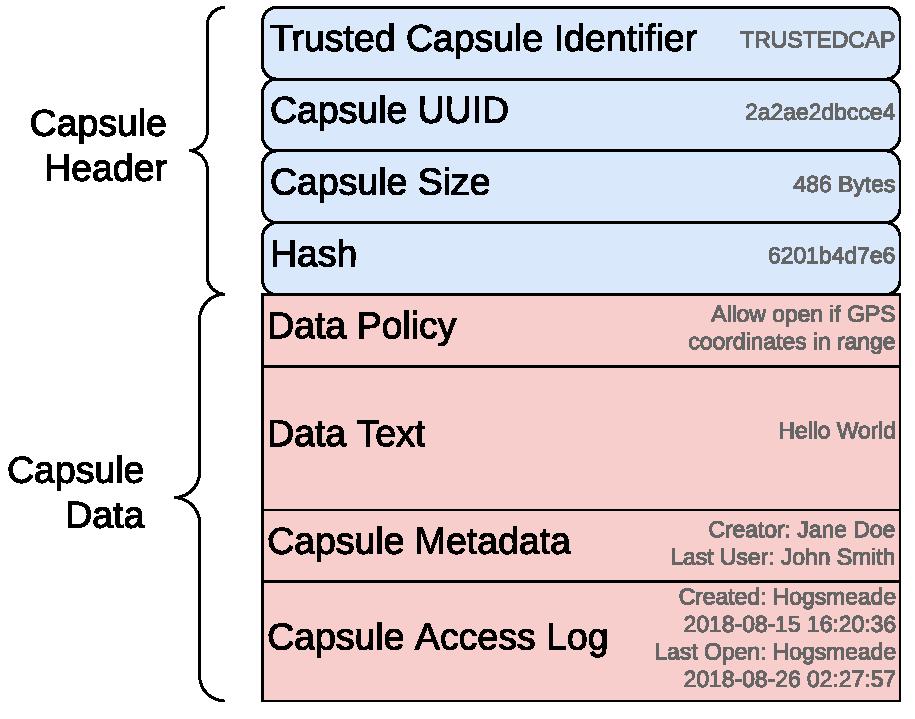
\includegraphics[width=\columnwidth]{fig/Fig2_Trusted_Capusle_Layout_New.pdf}
    \caption{Trusted capsule layout.}
    \label{fig:trustedcapsulelayout}
\end{figure}
%%%%%%%%%%%%%%%%%%%%

A capsule consists of data and an access policy for the data, both encapsulated
into a single encrypted file. Figure~\ref{fig:trustedcapsulelayout} illustrates
the format of a capsule. A capsule has an unencrypted header segment (Shown in blue in Figure~\ref{fig:trustedcapsulelayout}) followed by an
encrypted data block (Shown in pink in Figure~\ref{fig:trustedcapsulelayout}). The header identifies the file as a capsule and contains
integrity metadata used by the data monitor:
\begin{enumerate}
    \item \textbf{Trusted Capsule Identifier}: This is used to identify that the file being accessed is a capsule. This identifier spells \say{TRUSTEDCAP} in plaintext.
    \item \textbf{Capsule UUID}: This is a unique identifier that gets assigned to the capsule at the time of creation. This is used to find the decryption keys in TrustZone.
    \item \textbf{Capsule Size}: This field stores the size of the capsule in bytes. This is used to create communication buffers to pass the contents to the secure world.
    \item \textbf{Hash}: This field stores the hash of the data block of the capsule.
\end{enumerate}


The data block contains the following:
\begin{enumerate}
    \item \textbf{Data Policy}: This Lua Policy script that is run by the Policy Engine in TEE. This is written in accordance with the Policy API.
    \item \textbf{Data Text}: These are the exact contents of the file being encrypted.
    \item \textbf{Capsule Metadata}: This section is to hold any Key:Value based metadata that the Policy Engine might need to evaluate the policy.
    \item \textbf{Capsule Access Log}: This section holds the latest accesses to the capsule. Every time a capsule is accessed, an entry gets appended here.
\end{enumerate}

The cryptographic keys required to decrypt capsules are securely loaded into a secure storage area accessible only by the TEE. The protocol to securely load keys into the TEE is described in Chapter ~\ref{ch:device_key_reg}.
%
%\iv{Have to differentiate between on-open and on-close policies.}

\section{Policy API}
\label{subsec:policy}

\begin{table}[]
\centering
%\resizebox{\textwidth}{!}{%
\begin{tabular}{|p{7cm}|p{5cm}|}
\hline
 & \textbf{Description} \\ \hline
\multicolumn{2}{|l|}{\textbf{Open-Only}} \\ \hline
\texttt{redact}\textit{(start, end, replaceBytes}) & Replace byte range [start, end] of trusted capsule data with bytes replaceBytes. \\ \hline
\multicolumn{2}{|l|}{\textbf{Close-Only}} \\ \hline
\texttt{readNewCapsuleData}(\textit{offset, length}) & Return length bytes from offset of new trusted capsule data. \\ \hline
\texttt{newCapsuleLength}() & Return the length of new trusted capsule data. \\ \hline
\multicolumn{2}{|l|}{\textbf{Shared}} \\ \hline
\texttt{getState}(\textit{key, where}) & Get state mapped to key from where. \\ \hline
\texttt{setState}(\textit{key, val, where}) & Set state mapped to key to val in where. \\ \hline
\texttt{getLocation}(\textit{where}) & Get location of device from where. \\ \hline
\texttt{getTime}(\textit{where}) & Get current time from where. \\ \hline
\texttt{readOriginalCapsuleData}(\textit{offset, length}) & Return length bytes from offset of original trusted capsule data. \\ \hline
\texttt{originalCapsuleLength}() & Return the length of original trusted capsule data. \\ \hline
\texttt{deleteCapsule}() & Delete the trusted capsule. \\ \hline
\texttt{updatePolicy}() & Check for policy update with trusted capsule server. \\ \hline
\texttt{appendToBlacklist}(\textit{key, where}) & Append key to blacklist of where - used by log to prune states in where. \\ \hline
\texttt{removeFromBlacklist}(\textit{key, where}) & Remove key from blacklist of where. \\ \hline
\end{tabular}%
% }
\caption{The Lua-based API that policies in Trusted Capsules may use}
\label{Tbl:lua_ext}
\end{table}
    
In Trusted Capsules, policies are written in the Lua programming language and
have one simple requirement: they must implement an {\tt evaluate\_policy}({\em
        op}) function that is called when the capsule is being opened or closed; the
    {\em op} argument distinguishes between the two. There is a basic sanity check in the trusted application to ensure that the operation is valid - for example, the calling application cannot request a \texttt{close()} on a capsule that was never opened. In either case, the function
has to return a boolean value that is interpreted differently depending on the
operation. If it returns {\tt true} on a capsule open, the data is decrypted and
given to the normal world app. Otherwise, access is denied. On a capsule close,
returning {\tt true} means file modifications by the normal world app will be
kept while {\tt false} means they will be discarded. Policies may also use the
Trusted Capsules API listed in Table~\ref{Tbl:lua_ext} to easily perform common
operations:

\textbf{Storing state}: Policies may store and retrieve arbitrary state using
the state-oriented APIs such as {\tt getState} and {\tt setState}. When using
such methods, the policy must specify {\em where}
the state is to be kept. A policy may securely store state in the metadata space within
its capsule, in external secure storage, or at a remote server. If a policy
communicates with a remote server, the networking stack in the normal world
kernel is used to initiate the connection. However, as the OP-TEE OS includes
the mbed TLS library~\cite{mbed}, it is possible to safely make an HTTPS
connection from the secure world without trusting the normal world.

\textbf{Ensuring data integrity}: Our Lua policy provides APIs to retrieve the
original trusted capsule data at file open (read) and the new trusted capsule
data at file close (write). Using these APIs, data owners can express
policies that, for example, protect specific data regions from being
overwritten. %%  \ar{This explanation is incomplete. How exactly does one prevent
%% specific regions from being overwritten?}

\textbf{Redaction}: Selective policy-based disclosure of trusted capsule
contents is a key feature of trusted capsules. Using our byte-oriented
redaction API, data owners can express arbitrary data
transformations on regions of the data based on the environment and
the state of the device \emph{prior to} disclosing information to the normal world.  Examples
of data transformations include removing sensitive texts or blurring
images. %  \ar{Probably should merge this and data integrity section together.}

\textbf{Revocation}: A policy can specify revocation in two
ways. First, we provide APIs to allow policies to self-delete a trusted
capsule. When the \textit{deleteCapsule} API is called, we overwrite
the trusted capsule file with zeros\footnote{This is because the Linux OS does not
    delete the file until the file's reference count becomes zero}. We then
make an RPC call into the normal world to delete the file and destroy the
trusted capsule application session. Such a revocation is permanent.  Second, we
allow retroactive policy changes via the remote capsule server. In this
scenario, the policy specifies a condition under which \textit{updatePolicy} is
called. If a new policy exists at the trusted capsule server, it is downloaded
by the trusted world and replaces the prior policy. Policy changes are temporary as the owner
could always change the policy back. %% With trusted capsules, revocation can be gradual
%% based on user needs.
%% \ar{This portion is
%%   weak. The {\tt deleteCapsule} method is easily defeated. If someone sends me
%%   an email with a capsule and I find the capsule revoking itself, couldn't I
%%   just download a copy of the capsule again? What's the utility of
%%   deleteCapsule?}

\textbf{Logging}: We extended the Lua language with the ability to report
information to the remote capsule server. To enable logging on open and close, \textit{log\_open}
and \textit{log\_close} flags must be set to true, respectively.
By default, the Lua sandbox will report the location,
identity, time, and the operation. Additional local or capsule state information is
also logged, unless otherwise specified by the APIs \textit{appendToBlacklist}
and \textit{removeFromBlacklist}. The logs are written into the LOG section of
the trusted capsule.  If the section runs out of space, the logs are flushed to
the remote server and then overwritten. %% \ar{Is this necessary as a
%% separate paragraph? The access log isn't used for anything special, so why not
%% have it part of the {\tt getState} and {\tt setState} API? Alternatively, add
%% the logging API methods to the table and just highlight the usefulness of that
%% here.}


\section{Data monitor}
\label{subsec:data_monitor}
%%%%%%%%%%%%%%%%%%%%
\begin{figure}
    \centering
    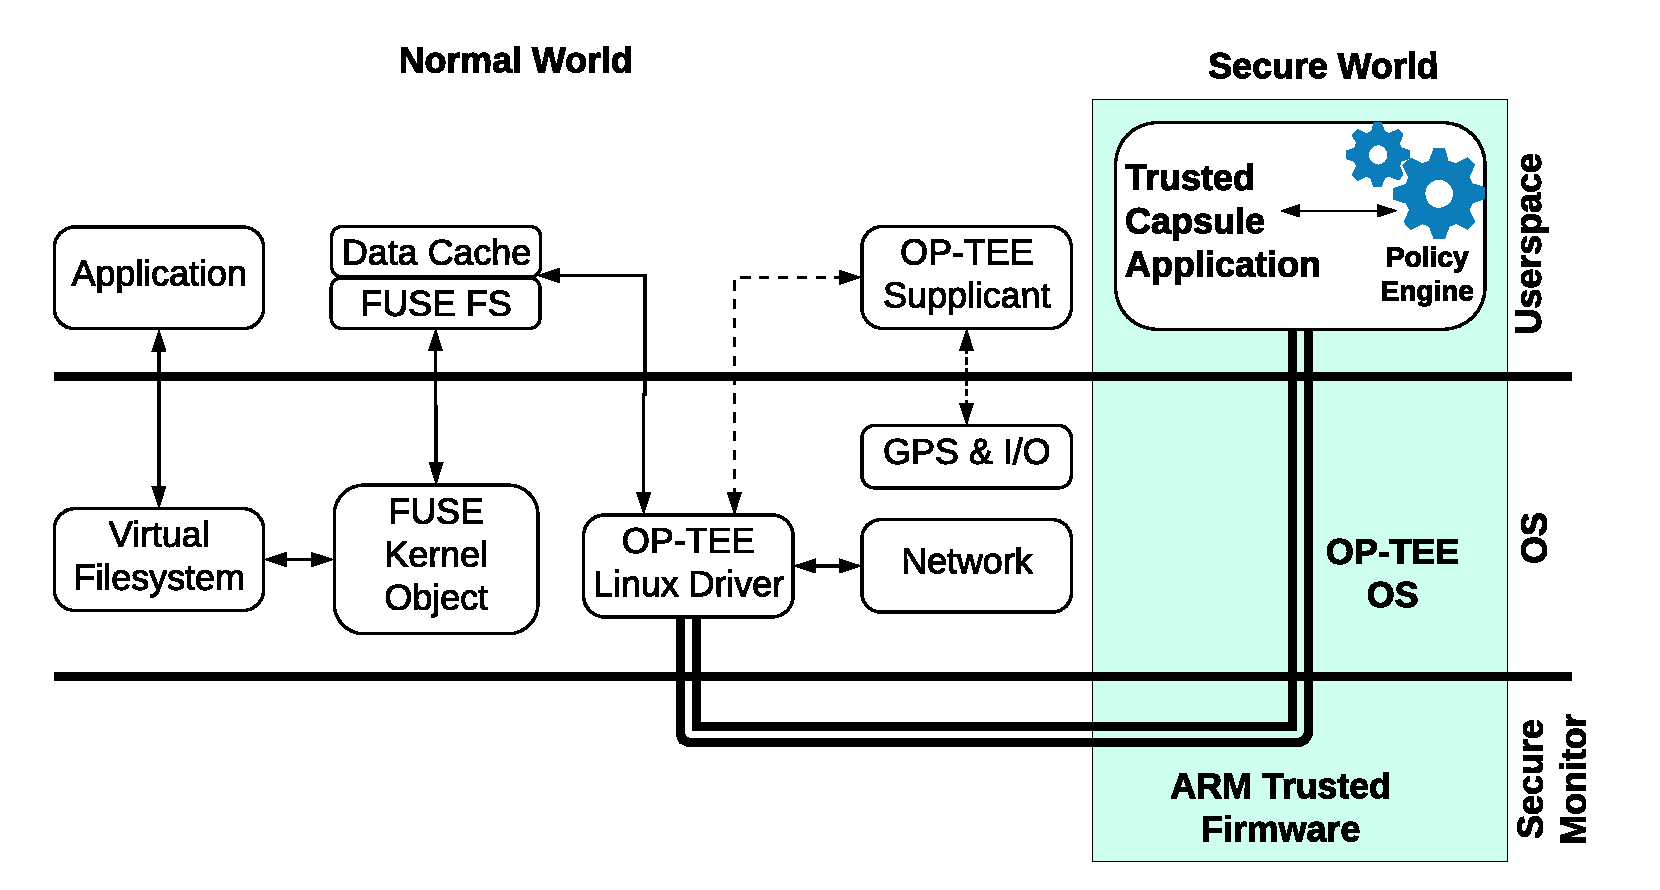
\includegraphics[width=\columnwidth]{fig/Fig3_TC_data_monitor_system_cache.pdf}
    \caption{Trusted capsule data monitor design. Application system calls to the filesystem for accessing trusted capsules are intercepted and forwarded to the trusted capsule application through the FUSE filesystem and OP-TEE Linux Driver.
        The secure world trusted capsule applications access peripheral I/O through RPC calls to the OP-TEE Supplicant via the OP-TEE Linux Driver.}
    \label{fig:SystemModel}
\end{figure}
%%%%%%%%%%%%%%%%%%%%

%%%%%%%%%%%%%%%%%%%%
\begin{figure*}
    \centering
    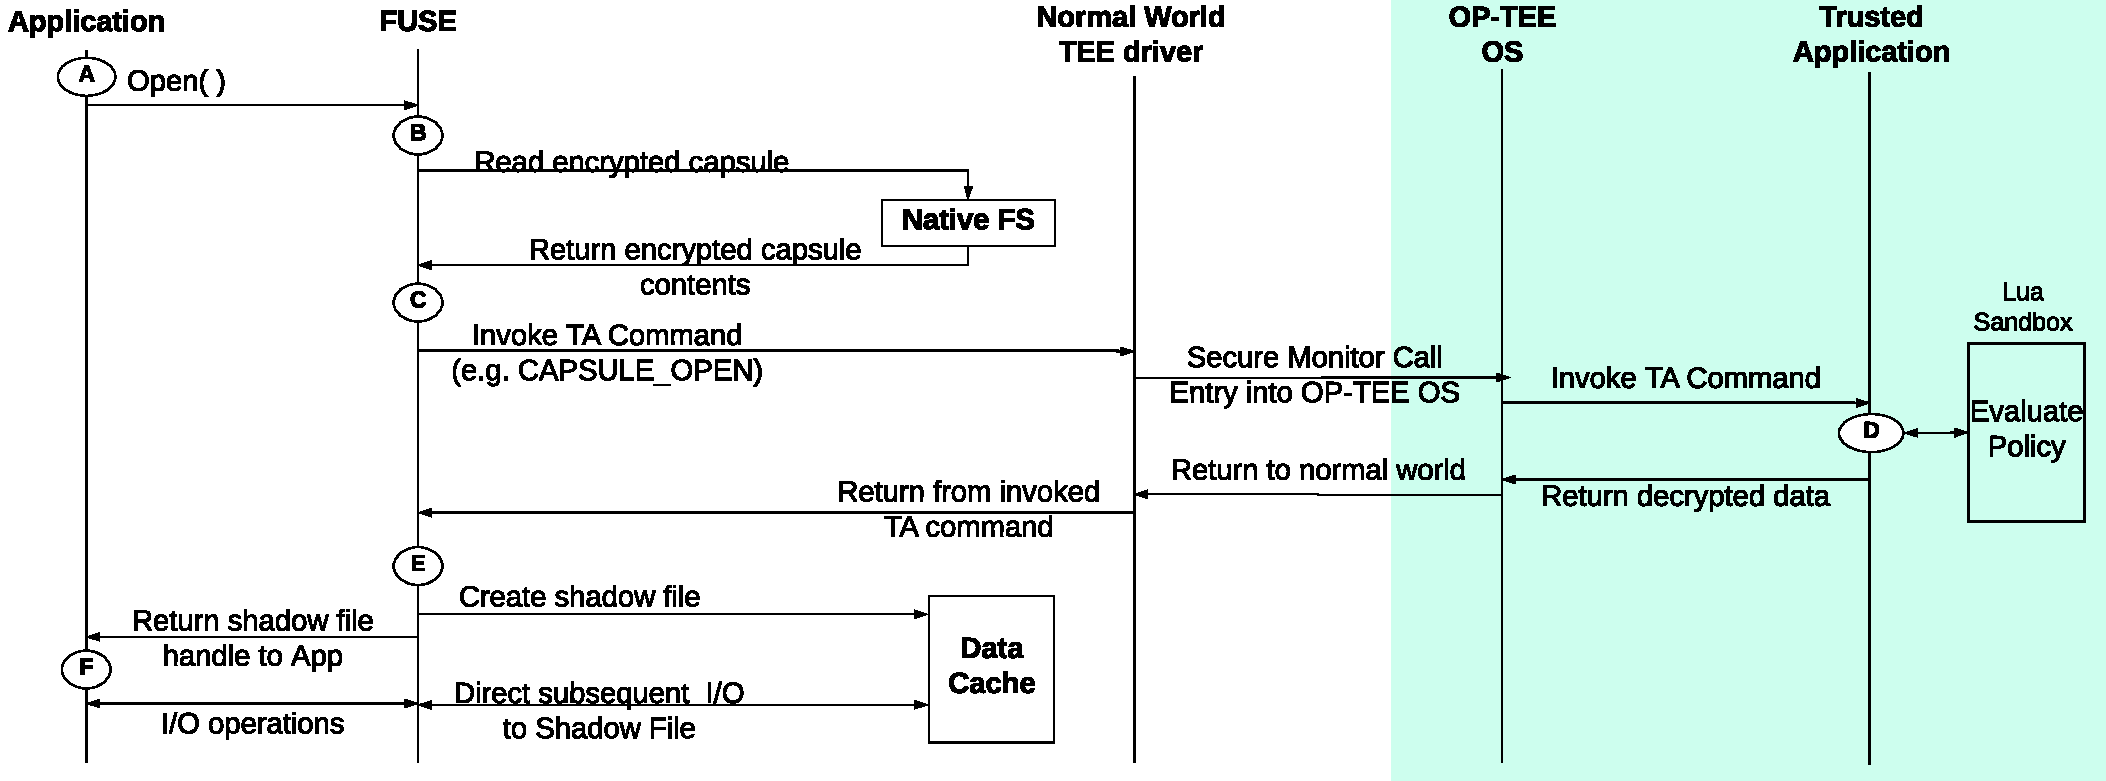
\includegraphics[width=\textwidth]{fig/TC_open_operation.pdf}
    \caption{Trusted capsule monitor operation (shaded region operates in the secure world).
        \textbf{A.} Application \textit{open} system call is intercepted.
        \textbf{B, C.} FUSE identifies if a file is a capsule, and if so, invokes an RPC into the secure world to decrypt the capsule.
        \textbf{D.} The trusted capsule application (TA) evaluates the \textit{open} policy.
        \textbf{E.} FUSE writes the decrypted contents to a shadow file
        \textbf{F.} The application is returned a filehandle to the shadow file, and all subsequent I/O requests are directed to the shadow file.
    }
    \label{fig:FlowChart}
\end{figure*}
%%%%%%%%%%%%%%%%%%%%

In Figure~\ref{fig:SystemModel}, we illustrate the different components of the
data monitor in our system and in Figure~\ref{fig:FlowChart}, we show a detailed
data flow between them when an application opens a capsule. These components may
be broadly classified into (1) framework code that runs in the normal world OS,
and (2) a policy execution engine in the secure world. Next, we discuss
each component in detail while referring to the data flow in
Figure~\ref{fig:FlowChart}.

{\bf Normal world framework}: We implemented a passthrough FUSE filesystem in
the normal world and expose it as a separate mount point. When an application
opens files located on this mount point, our framework will interpose on the
application's {\tt open} syscall. It will check the header of the file to
identify if it is a capsule. If it is a regular file, it will just load the raw
file from the underlying file system and return it to the app.

If it is a capsule, the file contents are copied into a memory buffer. FUSE then
shares this buffer with the policy execution engine running inside the secure world
and invokes the engine's {\em decrypt} function ({\em A}-{\em C} in
Figure~\ref{fig:FlowChart}). If the policy authorizes the access, the policy
engine will return the decrypted contents of the capsule and FUSE will save them
into a shadow file ({\em E}). It will subsequently return a handle to this
shadow file to the application ({\em F}). Hence, all reads and writes to the
capsule by the application will be transparently redirected to the shadow file.

When the application closes the capsule, FUSE copies the shadow file back into a
shared buffer, sends it to the policy execution engine, and invokes the {\em encrypt}
operation. This returns the reconstructed capsule, with the updated policy
metadata and data contents (as authorized by the policy), which is then written
in place of the original capsule file.

Our framework prevents multiple applications from concurrently opening the same
capsule. This simplifies the design of our data monitor as we do not have to
reason about multiple-reader/multiple-writer type problems when saving a
capsule. An application may, however, have multiple capsules open.

    {\bf Policy execution engine}: We implemented a Trusted Application (TA) that
runs in the secure world. It contains a Lua interpreter, to execute
a capsule's policies, and it is responsible for maintaining the runtime session
state associated with a capsule (e.g., cryptographic keys) and updating the
capsule metadata.

When a {\em decrypt} operation is received from the normal world (because a
normal world application used the {\tt open} syscall on a capsule), a new
instance of the trusted application is started. It (1) loads the capsule, (2)
loads the cryptographic keys for the capsule, (3) executes the policy, and (4)
returns the decrypted capsule data if authorized by the policy. During policy
evaluation, it may communicate to a remote server directly from the secure world.

On an {\em encrypt} operation (which is initiated because a normal world
application used the {\tt close} syscall to close a capsule), the TA evaluates
the policy and provides it the opportunity to allow or deny modifications to the
capsule data. Next, it updates the metadata, produces a new capsule file with
updated contents in the data block, and updates the integrity metadata in the
header. Finally, the reconstructed capsule is given to the normal world for
storage and subsequent use.

%%%%%%%%%%%%%%%%%%%%
% \begin{figure}
%   \centering
%   \includegraphics[width=\columnwidth]{../Images/TrustedApplicationSession.pdf}  
%   \caption{Trusted capsule monitor session model. Each Trusted Capsule Application maintains the session for
%            a single trusted capsule. It supports multiple file handles per trusted capsule. The file handles
%            consists of the process ID and file descriptor.}
%   \label{fig:trustedapplicationsession}
% \end{figure}
%%%%%%%%%%%%%%%%%%%%    

% Each instance of the trusted application independently maintains a trusted
% capsule's session state. \textbf{Session states include the \emph{cryptographic
%     and hashing handles, role-based credentials, hashes of the trusted capsule
%     contents, and copies of the data and policy}}. Further, the trusted
% application acts as the \textbf{endpoint for secure communication with a trusted
%   capsule server for performing remote functions} (e.g., fetching remote state
% or initiating a policy change). The trusted capsule application handles
% sensitive information and performs critical functions that must be protected
% against the untrusted normal world. Therefore we require this part of the
% trusted data monitor to execute within TrustZone.

We use OP-TEE OS native secure storage capability to store our cryptographic
keys and persistent trusted capsule states. The cryptographic information is stored
in serialized binary while trusted capsule states are stored in key-value
format. All trusted capsule encryption keys are stored in a single secure key
file. We allow the key file to be accessible by multiple trusted capsule
applications at a time so that multiple sessions can be instantiated
simultaneously to handle different capsules. In contrast, each capsule gets its
own secure state file. State files can only be opened by a single trusted
capsule application at a time. This is enforced through the OP-TEE OS. In this
way, we enforce a single trusted capsule instance at a time per capsule.

% Trusted application methods are invoked by FUSE-based on specific system
% calls. In this way, access control can be enforced dynamically based on the
% local and remote state when such a system call is initiated. We describe several
% of these methods below.

\section{Security analysis}

We consider two important security aspects of the Trusted Capsules data monitor.

\textbf{Trusted Capsules}: Operations on the trusted capsule are performed by
the trusted application in the secure world. We isolate each trusted capsule by
having separate instances of the trusted application handle each capsule and
by relying on OP-TEE OS to isolate each trusted application instance.
Our system stores persistent state associated with capsules (such as cryptographic keys)
in the secure storage functionality available in OP-TEE.

Given our use of TrustZone, the confidentiality and integrity of the capsule
data is protected against compromises of the normal world OS, particularly in
the pessimistic state. A compromised normal world OS may corrupt a capsule, but
that corruption will be detected during decryption. In the worst case, a compromised OS
may leak the data of capsules that are open during the compromise.

\textbf{Policy Evaluation}: To account for malicious policies, we made several
changes to the Lua interpreter to make it a sandbox. We disabled any Lua library
that allows the interpreter to interact with external systems (e.g., I/O,
packages, debug, and OS). We also extended the interpreter to prevent policies
from (1) interacting with any files other than the capsule, (2) from accessing
keys associated with other capsules, and (3) reading unauthorized device
peripherals. A malicious policy may attempt denial-of-service attacks such as
infinite loops. However, these may be addressed even by the normal world, by
canceling an {\em encrypt} or {\em decrypt} commands that do not complete after
some time.